\documentclass[12pt, openany, letterpaper]{memoir}
\usepackage{HomeworkStyle}

\begin{document}

\begin{center}
	{\large Homework 4 -- Physical Transformations of Pure Substances}
	
	Due: Monday, October 2 \hspace{3em} Points: ${\dfrac{~}{~~30~~}}$
\end{center}

Name: \rule[-.1mm]{15em}{0.1pt}

\begin{description}	
	\item [Exercise 4A.1(a)] ~ (5 points)
	
	How many phases are present at each of the points marked in Fig. 4.1a?
	
	\noindent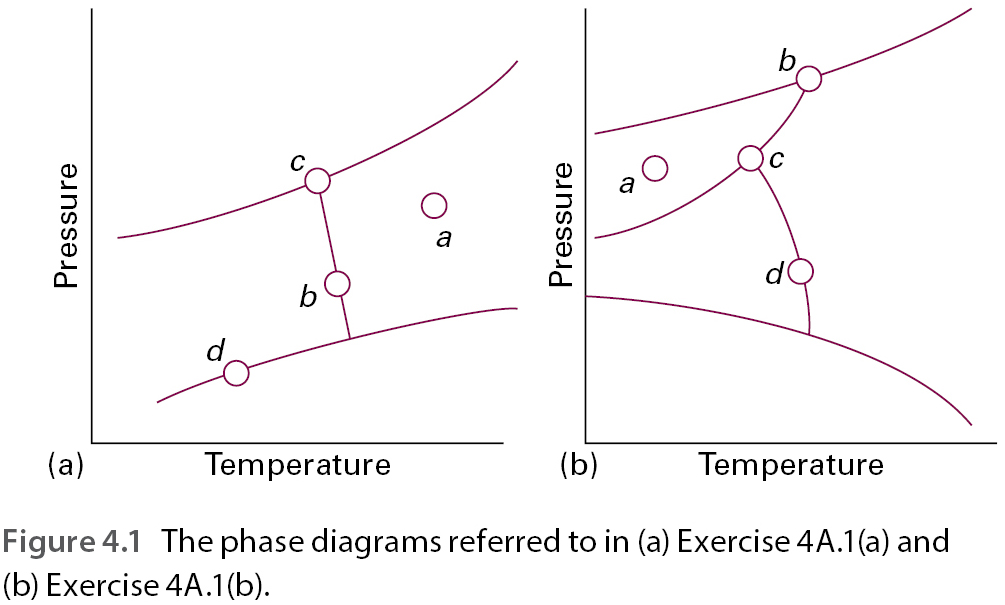
\includegraphics[width=0.5\linewidth]{Phase_Diagrams}
	\item [Exercise 4A.3(a)] ~ (5 points)
	
	What is the maximum number of phases that can be in mutual equilibrium in a two-component system?
	
	\vspace{10em}
	\item [Exercise 4B.6(a)] ~ (5 points)
	
	The vapour pressure of dichloromethane at $24.1^\circ C$ is $53.3~kPa$ and its enthalpy of vaporization is $28.7~\nicefrac{kJ}{mol}$. Estimate the temperature at which its vapour pressure is $70.0~kPa$.
	

	
	\vspace{10em}
	\item [Exercise 4B.8(a)] ~ (10 points)
	
	The vapour pressure of benzene between $10^\circ C$ and $30^\circ C$ fits the expression:
	
	 $\log_{10}~\nicefrac{p}{torr} = 7.960-\dfrac{\nicefrac{1780}{K}}{T}$ 
	 
	 Calculate (i) the enthalpy of vaporization and (ii) the normal boiling pont of benzene.
	
	\vspace{20em}
	\item [Exercise 4B.9(a)] ~ (5 points)
	
	When benzene freezes at $1.00~atm$ and $5.5^\circ C$ its density changes from $0.879~\nicefrac{g}{cm^3}$ to $0.891~\nicefrac{g}{cm^3}$. Its enthalpy of fusion is $10.59~\nicefrac{kJ}{mol}$. Estimate the freezing point of benzene at $1000.0~atm$.
	
	\vspace{15em}	
\end{description}
\end{document}